\documentclass[11pt, oneside]{article}   	% use "amsart" instead of "article" for AMSLaTeX format
\usepackage{geometry}                		% See geometry.pdf to learn the layout options. There are lots.
\geometry{a4paper}                   		% ... or a4paper or a5paper or ... 
%\geometry{landscape}				% Activate for for rotated page geometry
\usepackage[parfill]{parskip}			% Activate to begin paragraphs with an empty line rather than an indent
\usepackage{graphicx}				% Use pdf, png, jpg, or eps§ with pdflatex; use eps in DVI mode

\usepackage{amssymb}
\usepackage{mhchem}
\usepackage{gensymb}
\usepackage{textcomp}
\usepackage{braket}
\usepackage{amsmath}
\usepackage{paralist}				% Inline lists...

\title{600.438 Computational Genomics \\ Project Proposal}
\author{Sachi Sanghavi}

\begin{document}
\maketitle

\section{Motivation}

Aging is a universal biological process; and is known to be a major risk factor in diseases like type-2 diabetes, cancer, Alzheimer's disease, and more. However, the underlying molecular mechanisms of aging are still not well understood. This leaves the question ``Is aging genetically programmed?'' open for debate. Studying the association between aging and gene expression might give us some insights which could lead to novel treatments for treating age-related diseases.

We propose to study aging -- gene expression association in humans [in subcutaneous adipose tissue and whole blood tissue], and its link to disease.

\section{Background}

The study is based on Yang, \emph{et al.} (2015). The major difference is that we have \emph{more} samples for the same tissues. As as a result, it'd be interesting to compare our results.

\section{Aims and Methods}

\begin{enumerate}
\item Find age -- gene expression association and report it for top 100 genes for subcutaneous adipose tissue and whole blood tissue
	\begin{itemize}
	\item Use linear regression (correct for gender and top 3 genotype PCs, and ensure gene expression PCs have p-value $>0.05$), bootstrapping (remove 20\% low expressed genes), and permutation (estimate false positives).
	\end{itemize}
\item Functional annotation of aging genes [up- and down-regulated separately]
	\begin{itemize}
	\item Use David tools.
	\end{itemize}
\item Tissue specific link between aging genes and complex disease genes.
	\begin{itemize}
	\item Disease gene data compiled from NIH GWAS and OHIM using clustering.
	\item Fisher's test for aging -- diseases genes link.
	\end{itemize}
\item Compare results with Yang, \emph{et al.} (2015).
\end{enumerate}


\section{Data}

Gene expression data is taken from GTEx project v6 (PC values for top 3 genotypes are available; labeled C1, C2, and C3 in figure 1).

\begin{figure}[!h]
\center
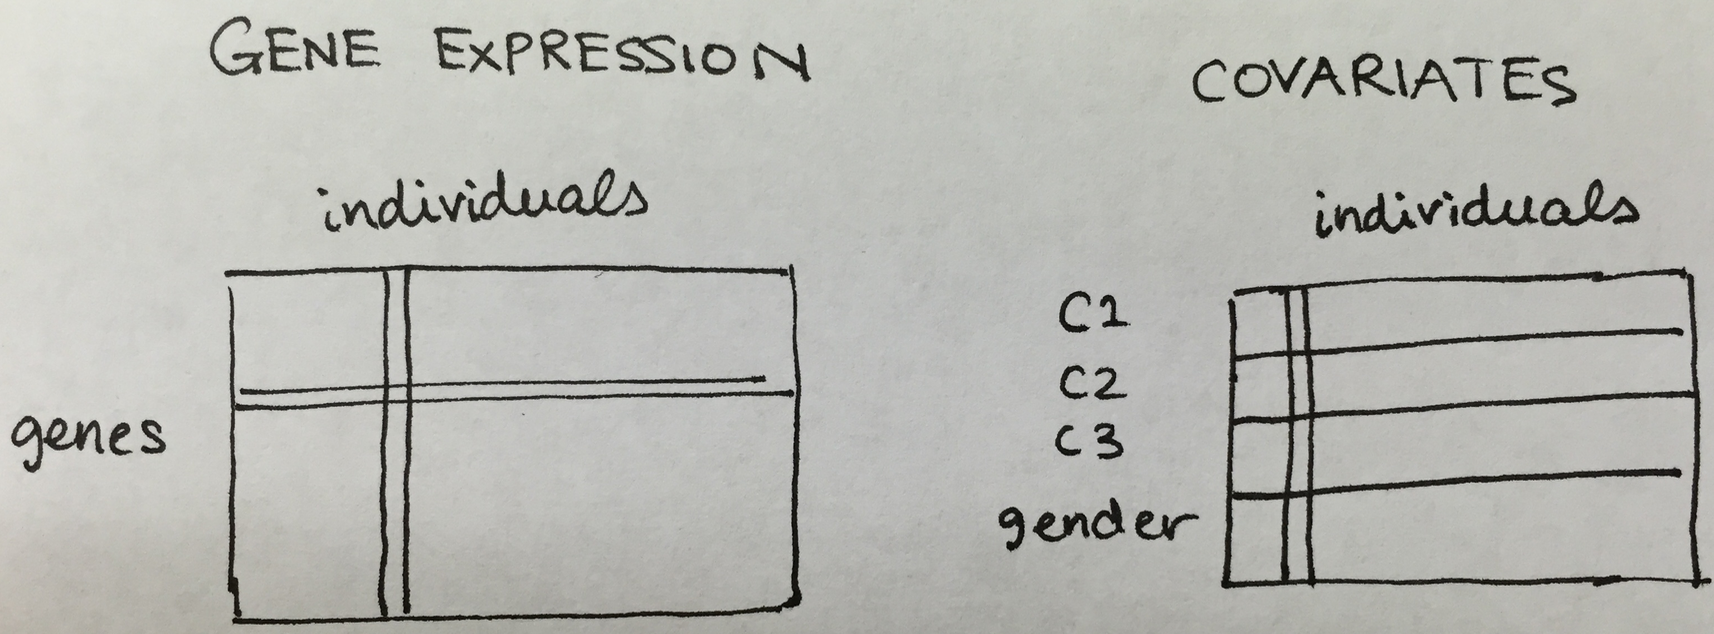
\includegraphics[width=12cm]{gtex}
\caption{Format of the two main data files from GTEx}
\end{figure}

\end{document}